\subsection*{U-Net Transformer: Self and Cross Attention for
Medical Image Segmentation}

% \subsection*{Ссылка} \url{https://arxiv.org/abs/2103.06104}
\subsubsection*{Введение}
Сегментация внутренних органов в медицине и компьютерной диагностике имеет 
колоссальное значение. На данный момент многие state-of-the-art методы 
опираются на полносвязные нейронные сети, такие как U-Net \cite{Unet} и ее разновидности. 
Несмотря на их хорошую производительность, полносвязные сети страдают от концептуальных 
ограничений в сложных задачах сегментации, например, сталкиваясь с визуальной 
неоднозначностью и низкой контрастностью органов.
\subsubsection*{Основная идея}
В данной работе \cite{ann19} предлагается сеть U-Transformer \cite{Unet}, которая использует 
сильные стороны трансформеров для моделирования далеко расположенные 
пространственные взаимоотношения между анатомическими структурами. U-Transformer 
сохраняет индуктивный сдвиг (inductive bias) светки с помощью U-Net подобной архитектуры, 
но включает в себя механизм внимания в двух главных слоях, который позволяет интерпретировать 
решения модели. Во-первых, self-attention модуль использует глобальне взаимоотношения между 
семантическими признаками на выходе энкодера, чтобы явно смоделировать полную контекстную информацию.
Во-вторых, представлен cross-attention в  скип-соединениях для фильтрации несемантических 
признаков, обеспечивая точное пространственное восстановление в U-Net декодере.
\\
\begin{minipage}{1.0\linewidth}
    \begin{center}
        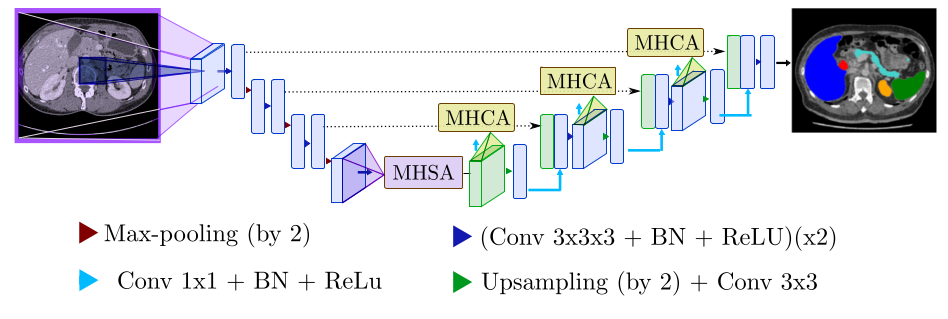
\includegraphics[scale=0.5]{ann19_arch.png} \\
        % \caption{\scriptsize{
        %     Архитектура U-Transformer.
        % }}
    \end{center}
    
\end{minipage} 
\subsection*{Данные}
TCIA - публичный датасет снимков поджелудочной железы.\\
Датасет снимков внутренних органов (IMO).
\subsection*{Результаты}

\begin{minipage}{1.0\linewidth}
    \begin{center}
        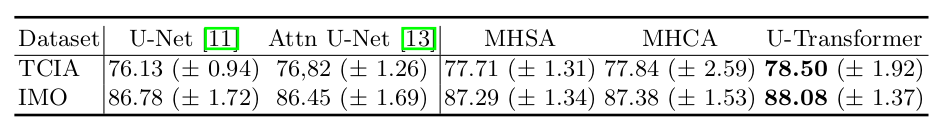
\includegraphics[scale=0.5]{ann19_res1.png} \\
        % \caption{\scriptsize{
        %     Результаты по метрике Dice.
        % }}
    \end{center}
    
\end{minipage}
\\
\\
\begin{minipage}{1.0\linewidth}
    \begin{center}
        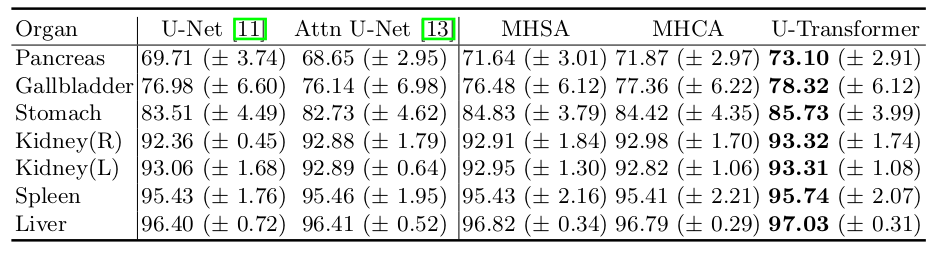
\includegraphics[scale=0.4]{ann19_res2.png} \\
        % \caption{\scriptsize{ 
        %      Результаты по каждому органу по метрике Dice на датасете IMO.}}
    \end{center}
    
\end{minipage} 

\subsubsection*{Заключение}
В данной работе была предложена сеть U-Transformer, которая расширяет U-Net подобную 
полносвязную сеть трансформером. Рассмотренный метод показывает лучщие результаты 
по сравнению с уже существующими решениями. В дальнейшем авторы планирую изучать 
U-Transformer'ы в трехмерном случае на снимках различной модальности.